\documentclass[]{article}
\title{Softwarearchitektur Übungsblatt 03}
\author{Marco Cotrotzo}
\usepackage{graphicx}
\usepackage{subfigure}
\date{}
\begin{document}
	\maketitle


\section{Aufgabe}
\renewcommand{\labelenumi}{\alph{enumi})}
\begin{enumerate}
\item

\textbf{ADP:}\\Acyclic-Dependencies-Prinzip sagt aus, dass keine Zyklen zwischen den Kompenenten entstehen soll. Da z.B Fehler in Zyklen schwerer gefunden werden können. Bei einer zyklischen Abhängigkeit können Auswirkungen, die durch Änderungen in der einen Komponente verursacht, schwerer durchblickt werden. \\

\textbf{SDP:}\\Stable-Dependencies-Prinzip.Stabile Kompnonenten sollten nur von stabileren Komponenten abhängig sein. Die Stabilität einer Komponente lässt sich mit positionaler Stabilität messen. Dabei errechnet man die Instabilität. \begin{center}
	\textbf{Instabilität $I = \frac{fanout}{fanout+fanin}$}
\end{center}
Fanin sind alle Komponenten außerhalb der betrachtenden Komponente, die von dieser Komponente abhängig sind. Alle eingehenden Abhängigkeiten.
Fanout sind alle Komponenten außerhalb der betrachtenden Komponente, von denen die betrachtenden Komponente abhängig ist. Alle ausgehenden Abhängigkeiten.\\
\\
\textbf{SAP:} \\Stable-Abstractions-Prinzip. Abhängigkeiten sollen in Richtung der Abstraktion verlaufen. Stabile Komponenten sollten aus abstrakten Klassen und Schnittstellen besetzen. Die Abhängigkeit einer Komponente lässt sich folgendermaßen bestimmen: 
\textbf{\begin{center}
		Abhängigkeit $A = \frac{Na}{Nc}$
\end{center}}
\textbf{Na:}\\ ...ist die Anzahl aller abstrakten Klassen und Interfaces einer Komponente.
\textbf{Nc:}\\ ...ist die Anzahl aller Klassen einer Komponente.
\\
\item 
\textbf{Architektur 1:}\\
\textbf{Presentation:}
Instabilität = $\frac{fanout}{fanin+fanout} = \frac{2}{0+2} = 1$ \\
Abstraktion = $\frac{Na}{Nc} = \frac{0}{2} = 0$\\
\textbf{Domain:}
Instabilität = $\frac{fanout}{fanin+fanout} = \frac{1}{2+1} = \frac{1}{3}$ \\
Abstraktion = $\frac{Na}{Nc} = \frac{0}{2} = 0$\\
\textbf{Infrastructure}
Instabilität = $\frac{fanout}{fanin+fanout} = \frac{0}{1+0} = 0$ \\
Abstraktion = $\frac{Na}{Nc} = \frac{0}{1} = 0$\\

\textbf{Architektur 2:}\\
\textbf{Presentation:}
Instabilität = $\frac{fanout}{fanin+fanout} = \frac{2}{0+2} = 1$ \\
Abstraktion = $\frac{Na}{Nc} = \frac{0}{2} = 0$\\
\textbf{Domain:}
Instabilität = $\frac{fanout}{fanin+fanout} = \frac{1}{2+1} = \frac{1}{3}$ \\
Abstraktion = $\frac{Na}{Nc} = \frac{1}{2} = \frac{1}{2}$\\
\textbf{Infrastructure}
Instabilität = $\frac{fanout}{fanin+fanout} = \frac{0}{1+0} = 0$ \\
Abstraktion = $\frac{Na}{Nc} = \frac{1}{2}\\$
\\

\begin{figure}
	\subfigure[Architektur 1]{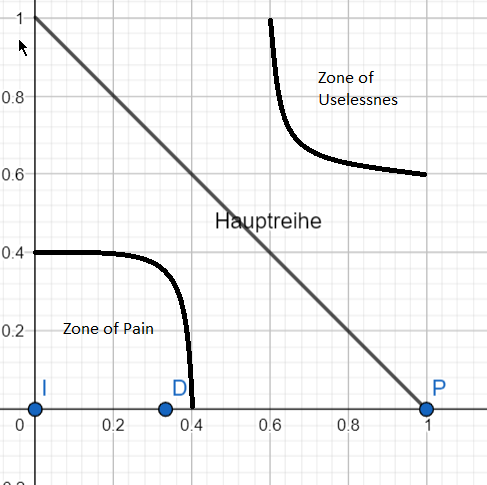
\includegraphics[width=0.49\textwidth]{Abbildung1IA.png}}
	\subfigure[Architektur 2]{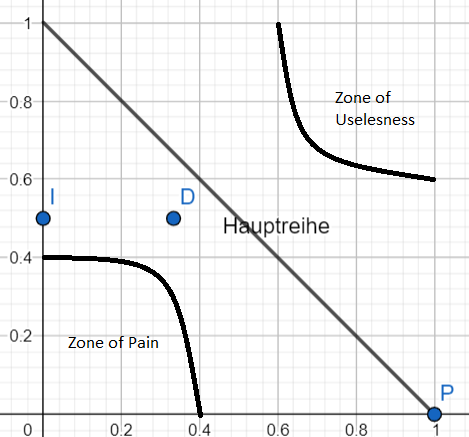
\includegraphics[width=0.49\textwidth]{Abbildung2.png}}
	\caption{I/A Graph}
\end{figure}
\item 
Bei der zweiten Architektur liegen die Komponenten Infrastructure und Domaine näher an der Hauptreihe. Bei der Infrastructure und Domaine wird mehr Abstraktion bei gleicher Stabilität erzielt. So wird das SAP-Prinzip besser eingehalten.  


\end{enumerate}
	
\end{document}